\documentclass[12pt, a4paper]{article}

\usepackage{ctex}
\usepackage{amsmath, amsthm, amssymb, mathrsfs, bm}
\usepackage{geometry}
\usepackage{graphicx}
\usepackage{hyperref}
\usepackage[numbers,sort&compress]{natbib}

\geometry{a4paper, left=2cm, right=2cm, top=2.5cm, bottom=2.5cm}

\setlength{\parindent}{2em}
\setlength{\parskip}{0.5em}
\allowdisplaybreaks[4]

\newtheorem{assumption}{假设}[section]
\newtheorem{definition}{定义}[section]
\newtheorem{theorem}{定理}[section]



% Mathematical notations
\newcommand{\R}{\mathbb{R}}
\newcommand{\E}{\mathbb{E}}
\newcommand{\Var}{\mathrm{Var}}
\newcommand{\Cov}{\mathrm{Cov}}

% Manifold notations
\newcommand{\manifold}{\mathcal{M}}
\newcommand{\metric}{g}
\newcommand{\dataspace}{\mathcal{X}}
\newcommand{\climatespace}{\mathcal{C}}
\newcommand{\measure}{P}
\newcommand{\attractor}{\mathcal{A}}

% 状态变量 (State Variables)
\newcommand{\fastvar}{\bm{x}}          % 快变量 (Fast Variables)
\newcommand{\slowvar}{\bm{c}}          % 慢变量 (Slow Variables)
\newcommand{\statespace}{\mathcal{S}}  % 状态空间 (State Space)

% 随机动力学 (Stochastic Dynamics)
\newcommand{\drift}{\mathcal{F}}  % 漂移向量场 (Drift Vector Field)
\newcommand{\diffop}{\sigma}      % 扩散算子 (Diffusion Operator)
\newcommand{\difftensor}{D}       % 扩散张量 (Diffusion Tensor)
\newcommand{\wiener}{W}           % 维纳过程 (Wiener Process)
\newcommand{\jacobian}{J}         % 雅可比矩阵 (Jacobian Matrix)
\newcommand{\fundsol}{M}          % 基本解矩阵 (Fundamental Solution Matrix)
\newcommand{\predtime}{\tau}      % 预报时间 (Prediction Time)

% 概率与统计 (Probability & Statistics)
\newcommand{\probdens}{p}           % 概率密度 (Probability Density)
\newcommand{\meanval}{\mu}          % 均值 (Mean)
\newcommand{\variance}{\sigma^2}    % 方差 (Variance)
\newcommand{\covmat}{\Sigma}        % 协方差矩阵 (Covariance Matrix)
\newcommand{\normdist}{\mathcal{N}} % 正态分布 (Normal Distribution)
\newcommand{\borel}{\mathcal{B}}    % Borel代数 (Borel Algebra)

% 特征值与特征向量 (Eigenvalues & Eigenvectors)
\newcommand{\eigenval}{\lambda}         % 特征值 (Eigenvalue)
\newcommand{\eigenvalmat}{\Lambda}      % 特征值矩阵 (Eigenvalue Matrix)
\newcommand{\diffeigenvalmat}{\Delta}   % 扩散特征值矩阵 (Diffusion Eigenvalue Matrix)
\newcommand{\eigenvecmat}{V}            % 特征向量矩阵 (Eigenvector Matrix)

% 几何与度量 (Geometry & Metric)
\newcommand{\manifolddim}{k}            % 流形维度 (Manifold Dimension)
\newcommand{\dyndist}{d}                % 动力学距离 (Dynamical Distance)
\newcommand{\evolop}{\phi}              % 演化算子 (Evolution Operator)
\newcommand{\coordmap}{\phi}            % 坐标映射 (Coordinate Map)
\newcommand{\mode}{\bm{\phi}}           % 主模态 (Principal Mode)

% 气候指标与阈值 (Climate Indicators & Thresholds)
\newcommand{\climind}{f}         % 气候指标/函数 (Climate Indicator/Function)
\newcommand{\threshold}{\theta}  % 阈值 (Threshold)



\title{\Large\textbf{地球系统的概率流形理论: 微分几何视角下的随机动力学过程}}
\author{刘滨瑞 \\ 地球系统科学系 \quad \href{mailto:lbr21@mails.tsinghua.edu.cn}{lbr21@mails.tsinghua.edu.cn}}
\date{\today}



\begin{document}

\maketitle

地球系统是一个典型的复杂系统，其状态空间维度高，时空尺度跨度大，确定性动力学与随机扰动深度耦合，存在着大量非线性的相互作用与反馈机制 \cite{wang2023earth}。
基于传统方法的研究难以刻画地球系统中发生的各种复杂过程，例如涌现、遥相关、模态转变等。
其根源在于缺乏统一的数学公理体系，不能描述地球系统的统计几何结构。

本文基于微分几何建立了\textbf{地球系统的概率流形理论}，将气候定义为参数化概率流形三元组 $(\manifold_{\slowvar}, \metric_{\slowvar}, \measure_{\slowvar})$。
理论基于三个核心洞察: 流形假设，由随机动力学过程诱导的不变概率测度，表征混沌效应与扩散过程的黎曼张量。

该理论框架将天气与气候、确定性与随机性统一在了一起，为地球系统建模构建了公理化的数学基础，能够具体解释地球系统中的多种特殊现象，可为模拟或预测研究提供新的思路。



\section{时间尺度分离}

地球系统跨越从毫秒到百万年的广泛时间尺度。
大气动力调整时间 (声波、重力波) 为分钟至小时，辐射平衡调整为周至月，海洋上层混合为月至年，深海环流为百年至千年，冰盖动力学为千年至万年 \cite{majda2012climate}。
这种时间上的多尺度性质源于系统的能量级联结构和不同物理过程的特征时间差异 \cite{arnold1998random}。

\begin{assumption}[时间尺度分离]
\label{ass:timescale_separation}
    地球系统的完整状态空间可分解为积空间 $\statespace = \dataspace \times \climatespace$，其中:
    \begin{itemize}
        \item 快变量 (Fast Variables): $\fastvar \in \dataspace \subset \R^N$: 大气温度、气压、风速、湿度、海表温度异常等在短时间尺度 ($\predtime_{\text{fast}} \sim 1$ 天至 $10$ 年) 内显著变化的状态分量。
        \item 慢变量 (Slow Variables): $\slowvar \in \climatespace \subset \R^M$: 大气$\text{CO}_2$ 浓度、太阳辐射、冰盖体积、地形等在长时间尺度 ($\predtime_{\text{slow}} \sim 10$ 年至 $10^6$年) 内缓慢演化的参数。
    \end{itemize}

    假设存在时间尺度分离条件:
    \begin{equation}
    \label{eq:timescale_separation}
        \epsilon = \frac{\predtime_{\text{fast}}}{\predtime_{\text{slow}}} \ll 1
    \end{equation}
\end{assumption}

当研究天气与短期气候 ($T \leq 10$ 年) 时，可将 $\slowvar$ 视为固定参数，因为慢变量在观测时间窗口内的变化相对于快变量可忽略。
当研究气候变化 ($T \geq 10$ 年) 时，需考虑 $\slowvar(t)$ 的缓慢演化及其对快变量动力学的影响。



\section{流形假设}

快变量 $\fastvar$ 所处的状态空间 $\dataspace = \R^N$ 的维度极高。
考虑 $1^\circ \times 1^\circ$ 网格、30层垂直、6个物理量 (温度、气压、比湿、三维风速)，则 $N = 360 \times 180 \times 30 \times 6 \approx 1.2 \times 10^6$，达到了百万量级。
经典统计学习理论 \cite{vapnik1999nature} 指出，样本复杂度随维度指数增长，即“维度灾难” (Curse of Dimensionality)。
即使我们有几十年的历史观测数据，样本点在如此高维的状态空间中也稀疏得可怜。
因此，理论上我们无法对 $\fastvar$ 进行任何有意义的统计分析。
幸运的是，维度灾难实际上并未阻止我们从事地球系统科学的研究。
其中的关键在于: \textbf{物理上可实现的状态并非均匀分布在整个状态空间 $\dataspace$ 中，而是受到严苛的约束条件，集中在某个低维子集上}。

具体而言，这些约束有:
\begin{itemize}
    \item \textbf{守恒律}: 质量守恒 $\nabla \cdot (\rho \bm{u}) + \frac{\partial \rho}{\partial t} = 0$，能量守恒，动量守恒；
    \item \textbf{动力学方程}: Navier-Stokes方程、热力学方程、连续性方程；
    \item \textbf{诊断关系}: 静力平衡 (大尺度运动)、地转平衡 (中高纬度)、状态方程 $p = \rho R T$；
    \item \textbf{边界条件}: 地表边界、大气顶、海陆分布；
    \item \textbf{物理可实现性}: $T, q, p > 0$，相对湿度 $\leq 100\%$，位温随高度变化受静力稳定性约束。
\end{itemize}

在微分几何学中，我们称 $\fastvar$ 被约束在一个\textbf{流形 (Manifold)}上，记作 $\manifold$。
不妨假定 $\manifold$ 是光滑的。

\begin{definition}[光滑流形]
\label{def:manifold}
    $\manifolddim$ 维光滑流形 $\manifold$ 是一个拓扑空间，配备图册 $A = \{(U_\alpha, \coordmap_\alpha)\}_{\alpha \in A}$，满足:
    \begin{itemize}
        \item 开覆盖: $\manifold = \bigcup_{\alpha} U_\alpha$；
        \item 局部同胚: 坐标图 $\coordmap_\alpha: U_\alpha \to V_\alpha \subset \R^{\manifolddim}$ 是同胚；
        \item 光滑转移: 转移映射 $\coordmap_\beta \circ \coordmap_\alpha^{-1}$ 是 $C^\infty$ 光滑的。
    \end{itemize}

    流形 $\manifold$ 可嵌入高维空间 $\dataspace$，存在嵌入映射 $\iota: \manifold \hookrightarrow \dataspace$。
\end{definition}

流形是可被“弯曲”但局部“平坦”的空间。
在任意点 $p \in \manifold$ 附近的小邻域，流形近似欧氏空间 $\R^k$，可用 $k$ 个坐标参数化。

\begin{definition}[切空间与流形维度]
\label{def:tangent_space}
    流形 $\manifold$ 在点 $p$ 处的切空间 $T_p\manifold$ 定义为:
    \begin{equation}
    \label{eq:tangent_space}
        T_p\manifold = \{\bm{v} \in \R^N : \bm{v} \perp N_p\manifold\}
    \end{equation}

    其中 $N_p\manifold$ 是法空间。
    $T_p\manifold$ 是由流形在 $p$ 点处的切向量张成的向量空间，是流形在 $p$ 点处的最佳线性逼近。
    流形的维数 $k$ 正是切空间的维数，它度量了流形的内在自由度。
\end{definition}

要想理解流形，我们可以想象一个嵌入在高维空间中的曲面，它可以被弯曲、扭转，但局部总是“平坦”的——任意小邻域都可以用 $k$ 个坐标参数化。

总结刚才的讨论，我们得出了一个深刻的洞察: 尽管观测空间的维度极高，但真实数据的内在自由度却往往很低。
在此基础上，我们提出了\textbf{流形假设 (Manifold Hypothesis)} \cite{fefferman2016testing}:

\begin{assumption}[流形假设]
\label{ass:manifold_hypothesis}
    固定慢变量 $\slowvar$，快变量 $\fastvar$ 嵌入于一个 $\manifolddim$ 维的光滑流形 $\manifold_{\slowvar} \subset \dataspace$ 上，其中 $\manifolddim \ll N$。
\end{assumption}

想象一张纸 (二维流形) 放在三维空间里。纸可以弯曲、折叠，但它本质上仍是二维的——你只需要两个坐标 (纸上的横坐标和纵坐标) 就能定位纸上的任意一点，尽管这张纸存在于三维空间中。
这就是“流形假设”: 我们所讨论的大气状态场，实际上就是高维状态空间 $\dataspace$ 中的一张“纸”。

考虑经验正交函数 (EOF)，对协方差矩阵 $\bm{C} = \frac{1}{n}\sum_{i=1}^N (\fastvar_i - \bar{\fastvar})(\fastvar_i - \bar{\fastvar})^\top$ 进行特征值分解，前 $K$ 个主成分的累积方差贡献率为:
\begin{equation}
\label{eq:eof_variance_contribution}
    r_K = \frac{\sum_{i=1}^K \eigenval_i}{\sum_{i=1}^N \eigenval_i}
\end{equation}

对于全球大气场，研究发现当 $K \sim 100$ 时，$r_K > 90\%$ \cite{hasselmann1988pips}。
这暗示大气子流形的内在维度约为 $10^2 \text{--} 10^3$，远小于 $N \sim 10^6$。
对于海洋子流形，主成分对应于一些气候模态: ENSO (第1-2模态，解释约40\%方差)、北大西洋涛动NAO、太平洋年代际振荡PDO、北极涛动AO等。
这些模态实际上就是流形的“坐标轴”，任意状态可近似表示为 $\fastvar \approx \bar{\fastvar} + \sum_{k=1}^K \alpha_k \mode_k$，其中$\{\mode_k\}$ 是主成分。

从动力学角度看，物理约束通过动力学过程持续将状态轨迹"拉回"流形。
如果因为某种原因产生了偏离流形的状态 (如负湿度)，快速调整过程 (声波、重力波、湍流混合) 会在短时间内将系统恢复至流形上。
因此，流形具有吸引性，它是动力系统演化的不变集 \cite{ghil2008climate}。

慢变量 $\slowvar$ 改变时，约束本身发生变化，流形 $\manifold_{\slowvar}$ 随之变化。
例如，$\text{CO}_2$ 的增加将改变辐射平衡，温度上升将导致饱和水汽压增加，从而改变了湿度的可实现范围。
这体现为流形在相空间中的“移动”或“变形”。



\section{参数化随机动力学与概率测度}

\subsection{伊藤随机微分方程}

在固定慢变量 $\slowvar$ 下，快变量 $\fastvar_t$ 的演化并不是确定性的。
次网格过程 (湍流、对流、云微物理等) 无法被精确模拟，只能使用参数化方案进行统计性描述。

\begin{assumption}[参数化随机动力学]
\label{ass:stochastic_dynamics}
    快变量 $\fastvar_t \in \manifold$ 的演化遵循伊藤随机微分方程 (Itô SDE) \cite{pavliotis2014stochastic}:
    \begin{equation}
    \label{eq:sde}
        d\fastvar_t = \drift(\fastvar_t; \slowvar)\,dt + \diffop(\fastvar_t; \slowvar)\,d\wiener_t
    \end{equation}

    其中:
    \begin{itemize}
        \item $\drift: \manifold \to T\manifold$ 是漂移向量场 (Drift Vector Field)，描述可解析尺度的确定性动力学；
        \item $\wiener_t \in \R^d$ 是 $d$ 维标准维纳过程 (Wiener Process)，满足 $\E[d\wiener_t] = 0$，$\E[d\wiener_t, d\wiener_t^\top] = I_d\,dt$；
        \item $\diffop: \manifold \to \mathcal{L}(\R^d, T\manifold)$ 是扩散算子 (Diffusion Operator)，将 $\wiener_t$ 线性映射为切空间中的随机扰动；
        \item $\difftensor(\fastvar; \slowvar) = \diffop(\fastvar; \slowvar)\diffop(\fastvar; \slowvar)^\top \in \R^{N \times N}$ 是扩散张量 (Diffusion Tensor)，对称正定，描述随机扰动的协方差结构。
    \end{itemize}
\end{assumption}

我们逐个解释Itô SDE中各项的物理意义:

\textbf{(1) 漂移项 $\drift(\fastvar; \slowvar)$}:
表示网格尺度可解析的物理过程，以及通过参数化方案统计性解析的次网格过程的系统性影响，如对流的净加热、湍流的平均应力。

\textbf{(2) 扩散项 $\diffop(\fastvar; \slowvar)\,d\wiener_t$}:
表示次网格过程的随机波动。
单个对流单体、湍流涡旋的生消是混沌的，无法显式跟踪。
在排除系统性影响后，我们可以用随机过程描述其随机性。
扩散张量 $\difftensor(\fastvar; \slowvar)$ 的对角元 $\difftensor_{ii}$ 表示第 $i$ 个自由度的随机扰动强度，非对角元 $\difftensor_{ij}$ 表示不同自由度的随机扰动相关性。

\textbf{(3) 维纳过程的维度 $d$}:
$d$ 是独立随机源的数量，物理上可理解为主导的随机模态数 (如不同波数的湍流模态)。
扩散算子 $\diffop \in \R^{N \times d}$ 将 $d$ 维随机源映射为 $N$ 维状态扰动，通常 $d \ll N$。

方程 \eqref{eq:sde} 定义了一个马尔可夫过程 (Markov Process): 未来演化只依赖当前状态 $\fastvar_t$，与过去路径无关。
这假设扩散项的记忆时间远小于漂移项的演化时间，即认为随机扰动无自相关 (白噪声近似) 。

\subsection{Fokker-Planck方程与稳态测度}

由 \eqref{eq:sde} 定义的马尔可夫过程，转移概率密度 $\probdens(\fastvar_t | \fastvar_0)$ 的演化满足Fokker-Planck方程 \cite{gardiner2009stochastic}:

\begin{theorem}[Fokker-Planck方程]
\label{thm:fp}
    设 $\probdens(\fastvar_t | \fastvar_0)$ 是从初始状态 $\fastvar_0$ 出发，在时刻 $t$ 位于 $\fastvar$ 的概率密度函数，则:
    \begin{equation}
    \label{eq:fp}
        \frac{\partial \probdens}{\partial t} = -\sum_{i=1}^N \frac{\partial}{\partial x_i}(\drift_i(\fastvar; \slowvar) \probdens) + \frac{1}{2}\sum_{i,j=1}^N \frac{\partial^2}{\partial x_i \partial x_j}(\difftensor_{ij}(\fastvar; \slowvar) \probdens)
    \end{equation}

    其中 $\drift_i$ 是漂移向量场的第 $i$ 个分量，$\difftensor_{ij} = [\diffop\diffop^\top]_{ij}$ 是扩散张量的分量。
\end{theorem}

方程 \eqref{eq:fp} 描述概率密度在状态空间的“流动”:
\begin{itemize}
    \item 漂移项 $-\sum_{i=1}^N \frac{\partial}{\partial x_i}(\drift_i(\fastvar; \slowvar) \probdens)$ 是平流效应，概率云被确定性向量场 $\drift(\fastvar; \slowvar)$ 推动；
    \item 扩散项 $\frac{1}{2}\sum_{i,j} \frac{\partial^2}{\partial x_i \partial x_j}(\difftensor_{ij}(\fastvar; \slowvar) \probdens)$ 是扩散效应，概率云因随机扰动而展宽。
\end{itemize}

\begin{assumption}[稳态测度的存在性]
\label{ass:stationary_measure}
    对固定的 $\slowvar$，假设SDE \eqref{eq:sde} 存在唯一的不变概率测度 $\measure_{\slowvar}$，其密度 $\probdens_{ss}(\fastvar; \slowvar)$ 满足稳态Fokker-Planck方程:
    \begin{equation}
    \label{eq:steady_fp}
        \frac{\partial \probdens_{ss}}{\partial t} = -\sum_{i=1}^N \frac{\partial}{\partial x_i}(\drift_i(\fastvar; \slowvar) \probdens_{ss}) + \frac{1}{2}\sum_{i,j=1}^N \frac{\partial^2}{\partial x_i \partial x_j}(\difftensor_{ij}(\fastvar; \slowvar) \probdens_{ss}) = 0
    \end{equation}
\end{assumption}

\begin{definition}[概率测度]
\label{def:probability_measure}
    对固定的 $\slowvar$，概率测度 $\measure_{\slowvar}$ 由稳态密度 $\probdens_{ss}(\fastvar; \slowvar)$ 定义:
    \begin{equation}
    \label{eq:probability_measure}
        \measure_{\slowvar}(A) = \int_A \probdens_{ss}(\fastvar; \slowvar)\,d\fastvar, \quad \forall A \in \borel(\manifold)
    \end{equation}

    其中 $\borel(\manifold)$ 是流形的Borel$\sigma$-代数。
\end{definition}

\begin{assumption}[遍历性]
\label{ass:ergodicity}
    假设马尔可夫过程 $\{\fastvar_t\}$ 在不变概率测度 $\measure_{\slowvar}$ 下是遍历的，即对任意可测函数 $\climind: \manifold \to \R$:
    \begin{equation}
    \label{eq:ergodic}
        \lim_{T \to \infty} \frac{1}{T}\int_0^T \climind(\fastvar_t)\,dt = \int_{\manifold} \climind(\fastvar)\,d\measure_{\slowvar}(\fastvar), \quad \text{几乎处处成立}
    \end{equation}
\end{assumption}

遍历性保证了时间平均和空间平均的等价性，是统计力学的基石 \cite{eckmann1985ergodic}。
想象一个粒子在流形 $\manifold$ 上遵循SDE \eqref{eq:sde} 进行随机游走，给定足够长的时间，粒子会“走遍”流形的每个位置，在任意区域 $A$ 停留的时间比例 $\approx \measure_{\slowvar}(A)$。
除了零测集外，不存在粒子“永远无法到达”或“永远困在其中”的区域。

在地球科学的实际观测中，我们通常只能获得一条时间序列——比如某个气象站40年的逐日温度记录。
遍历性告诉我们: 这一条长时间序列的期望值趋近于真实的期望值，即温度的气候态。
也就是说，\textbf{我们可以用对系统的长时间观察代替随机采样}。

事实上，假设 \ref{ass:stationary_measure} 和 \ref{ass:ergodicity} 在如下条件下可被严格证明 \cite{hairer2006ergodic}:
\begin{enumerate}
    \item 一致椭圆性: 扩散张量 $\difftensor(\fastvar; \slowvar)$ 处处非退化，即 $\exists \eigenval_{\min} > 0$ 使得 $\bm{\xi}^\top \difftensor(\fastvar; \slowvar) \bm{\xi} \geq \eigenval_{\min} \|\bm{\xi}\|^2$ 对所有 $\fastvar \in \manifold$ 和 $\bm{\xi} \in \R^N$ 成立；
    \item 次线性增长条件: $\exists C > 0$ 使得 $\|\drift(\fastvar; \slowvar)\| \leq C(1 + \|\fastvar\|)$ 对所有 $\fastvar \in \manifold$ 成立；
    \item 耗散性: $\exists \alpha, \beta > 0$ 使得 $\langle \drift(\fastvar; \slowvar), \fastvar \rangle \leq -\alpha \|\fastvar\|^2 + \beta$ 对充分大的 $\|\fastvar\|$ 成立。
\end{enumerate}

对于地球系统而言，这些条件在物理上具有合理性:
\begin{itemize}
    \item 条件 (1) 要求次网格随机扰动处处非零 (湍流、对流过程无处不在)；
    \item 条件 (2) 要求物理量不会无限增长 (温度、风速存在能量上界约束)；
    \item 条件 (3) 要求存在能量耗散机制 (摩擦、辐射冷却、边界层拖曳)。
\end{itemize}



\section{混沌与扩散: 黎曼度量}

\subsection{Lipschitz连续性}

为了在流形 $\manifold$ 上定义距离、角度、体积、曲率等几何概念，我们定义\textbf{度量张量 (Metric Tensor)} $\metric$。

\begin{definition}[度量张量]
\label{def:metric_tensor}
    度量张量 $g$ 是定义在流形切丛上的一个光滑、对称、正定的 $(0, 2)$ 型张量场。在局部坐标 $\bm{u} = (u^1, \ldots, u^k)$ 下，它表示为对称正定矩阵 $[\metric_{ij}(\bm{u})]$。
    两个无穷接近的点之间的距离平方为:
    \begin{equation}
    \label{eq:metric_tensor_def}
        ds^2 = \sum_{i,j=1}^k g_{ij}(\bm{u})\,du^i\,du^j = d\bm{u}^\top \metric(\bm{u}) d\bm{u}
    \end{equation}
\end{definition}

基于度量张量 $\metric$，我们定义\textbf{测地距离 (Geodesic Distance)} $d_\metric$。

\begin{definition}[测地距离]
\label{def:geodesic_distance}
    给定度量张量 $\metric$，流形 $\manifold$ 上两点 $p, q$ 之间的测地距离 $d_\metric(p, q)$ 定义为:
    \begin{equation}
    \label{eq:geodesic_distance}
        d_\metric(p, q) = \inf_{\gamma: p \to q} \int_0^1 \sqrt{\sum_{i,j=1}^k \metric_{ij}(\gamma(t)) \dot{\gamma}^i(t) \dot{\gamma}^j(t)}\, dt
    \end{equation}

    其中 $\gamma: [0,1] \to \manifold$ 是连接 $p = \gamma(0)$ 和 $q = \gamma(1)$ 的光滑曲线，$\dot{\gamma}(t) = \frac{d\gamma}{dt}$ 是切向量。
    测地距离是所有连接 $p$ 和 $q$ 的曲线中最短的弧长。
\end{definition}

我们定义\textbf{曲率 (Curvature)} 来刻画流形的弯曲程度 \cite{lee2018introduction}。

\begin{definition}[Riemann曲率张量]
\label{def:riemann_curvature_tensor}
    \begin{equation}
    \label{eq:riemann_curvature_tensor}
        R_{ijkl} = \frac{\partial \Gamma_{il}^m}{\partial x^k} - \frac{\partial \Gamma_{ik}^m}{\partial x^l} + \Gamma_{il}^n\Gamma_{nk}^m - \Gamma_{ik}^n\Gamma_{nl}^m
    \end{equation}

    其中 $\Gamma_{jk}^i = \frac{1}{2}g^{im}(\frac{\partial g_{mj}}{\partial x^k} + \frac{\partial g_{mk}}{\partial x^j} - \frac{\partial g_{jk}}{\partial x^m})$ 是Christoffel符号。
\end{definition}

通过对Riemann曲率张量进行收缩，可得到Ricci曲率张量: $\mathrm{Ric}_{ij} = R_{ikjl}g^{kl}$。
进一步收缩，得到\textbf{标量曲率}: $R = \mathrm{Ric}_{ij}g^{ij}$。
标量曲率 $R$ 可近似理解为度量张量的二阶变化:
\begin{equation}
\label{eq:scalar_curvature_approximation}
    R \sim \|\nabla^2 g\|
\end{equation}

\textbf{近邻假设 (Neighborhood Preserving)} 认为: \textbf{在流形上距离相近的点，其演化行为应该是类似的}。
考虑演化算子 $\evolop_t: \manifold \to \manifold$，$\evolop_t(\fastvar_0) = \fastvar(t)$。
一个好的度量 $\dyndist_\metric$ 应使 $\evolop_t$ 具有小的Lipschitz常数 $L$:
\begin{equation}
\label{eq:neighborhood_preserving}
    \dyndist_\metric(\evolop_t(\fastvar_A), \evolop_t(\fastvar_B)) \leq L \cdot \dyndist_\metric(\fastvar_A, \fastvar_B), \quad \forall \fastvar_A, \fastvar_B \in \manifold
\end{equation}

在尝试拟合演化算子 $\evolop_t$ 时，Lipschitz平滑性 \eqref{eq:neighborhood_preserving} 将带来以下好处:
\begin{itemize}
    \item 稳定性 (Stability): 模型具有更高的可预报性极限；
    \item 泛化性 (Generalization): 模型在训练样本的“近邻”内泛化误差可控，预测可靠性高；
    \item 正则化 (Regularization): 较小的Lipschitz常数隐含正则化条件，可以防止模型过拟合；
    \item 鲁棒性 (Robustness): 模型能够容忍一定的观测误差和数值误差。
\end{itemize}

因此，如何构造符合近邻假设，具有较好Lipschitz平滑性的度量 $\metric$，是一个十分重要的问题。
欧氏距离 $\dyndist_{\text{Euclid}}(\fastvar_A, \fastvar_B) = \|\fastvar_A - \fastvar_B\|_2$ 显然不是一个好的选择——物理上相似的状态在欧氏距离下可能很远，物理上差异巨大的状态反而接近。
这里举一个具体例子，我们考虑两个扰动:
\begin{itemize}
    \item 扰动A: ENSO核心区 (约占全球面积的 1\%) 的0.5K海温异常。
    \item 扰动B: 全球每个格点均匀的0.01K温度扰动。
\end{itemize}

按照欧式距离，扰动B的影响更大，即扰动前后状态的距离更远，相似性更低。
但从气候动力学角度理解: 扰动A会在数周内通过Walker环流以遥相关的方式影响全球天气，而扰动B几乎不会产生任何影响。
这说明欧氏距离给出了错误的相似性判断。
如果我们基于此进行建模，模型会认为扰动B的效果“更显著”，这与物理实际完全相反。

\subsection{动力学距离}

Itô SDE \eqref{eq:sde} 描述的动力学系统是随机的。
从一个初始状态 $\fastvar_0$ 出发，系统在未来 $t$ 时刻的状态 $\fastvar(t)$ 服从概率分布 $\probdens_t(\cdot | \fastvar_0)$。
根据近邻假设，\textbf{动力学相似性应由未来状态分布的差异来衡量}。

\begin{definition}[动力学距离]
\label{def:tau_distance}
    固定预报时间 $\predtime > 0$，两初值 $\fastvar_A, \fastvar_B$ 的动力学距离定义为:
    \begin{equation}
    \label{eq:tau_distance}
        \dyndist_{\predtime}(\fastvar_A, \fastvar_B) = \sqrt{\predtime} \cdot d_p(\probdens_{\predtime}(\cdot | \fastvar_A), \probdens_{\predtime}(\cdot | \fastvar_B))
    \end{equation}

    其中 $d_p$ 是某个量化概率分布差异的距离函数，如Wasserstein距离 \cite{villani2009optimal}。
    时间权重因子 $\sqrt{\predtime}$ 反映了预报时间对距离度量的自然贡献。
\end{definition}

为推导 $\dyndist_{\predtime}$ 的显式形式，需要分析\textbf{SDE的有限时间演化}。
考虑相邻初值 $\fastvar_A, \fastvar_B$，记 $\delta\fastvar_0 = \fastvar_B - \fastvar_A$ 为初始扰动。
我们提出以下假设:

\begin{assumption}[局部平稳扩散]
\label{ass:local_stationary_diffusion}
    扩散算子 $\diffop(\fastvar)$ 在小邻域内近似常数:
    \begin{equation}
    \label{eq:local_stationary_diffusion}
        \diffop(\fastvar+\delta\fastvar) \approx \diffop(\fastvar)
    \end{equation}
\end{assumption}

\begin{assumption}[局部线性化]
\label{ass:local_linearization}
    在初值的小邻域 $\|\delta\fastvar_0\|$ 内，漂移项可线性化:
    \begin{equation}
    \label{eq:local_linearization}
        \drift(\fastvar + \delta\fastvar) \approx \drift(\fastvar) + \jacobian_{\drift}(\fastvar) \delta\fastvar
    \end{equation}

    其中 $\jacobian_{\drift} = \frac{\partial \drift}{\partial \fastvar}$ 是雅可比矩阵。
\end{assumption}

\begin{assumption}[适度时间尺度]
\label{ass:moderate_time_scale}
    预报时间 $\predtime$ 满足:
    \begin{equation}
    \label{eq:moderate_time_scale}
        \predtime \ll \frac{1}{\|\jacobian_{\drift}\|} \cdot \frac{L}{\|\delta\fastvar_0\|}
    \end{equation}

    其中 $L$ 是系统特征尺度。这保证线性近似在 $[0, \predtime]$ 内有效。
\end{assumption}

在以上假设下，扰动的演化满足线性化SDE:
\begin{equation}
\label{eq:linearized_sde}
    d(\delta\fastvar_t) = \jacobian_{\drift}(\fastvar_t) \delta\fastvar_t\,dt + \diffop(\fastvar_t) d\wiener_t
\end{equation}

为进一步简化，我们假设动力学场在预报时间 $\predtime$ 内缓慢变化:

\begin{assumption}[缓变场假设]
\label{ass:slowly_varying_fields}
    雅可比矩阵 $\jacobian_{\drift}(\fastvar_t)$ 和扩散算子 $\diffop(\fastvar_t)$ 在时间尺度 $\predtime$ 内近似常数:
    \begin{equation}
    \label{eq:slowly_varying_fields}
        \jacobian_{\drift}(\fastvar_t) \approx \jacobian_{\drift}(\fastvar_0), \quad \diffop(\fastvar_t) \approx \diffop(\fastvar_0), \quad \forall t \in [0, \predtime]
    \end{equation}
\end{assumption}

考虑从初值 $\fastvar_A$ 和 $\fastvar_B = \fastvar_A + \delta\fastvar_0$ 出发的两条轨迹。
在假设 \ref{ass:slowly_varying_fields} 下，线性化SDE \eqref{eq:linearized_sde} 是常系数的，其解为:
\begin{equation}
\label{eq:perturbation_solution}
    \delta\fastvar_t = \fundsol_t \delta\fastvar_0 + \int_0^t \fundsol_{t-s} \diffop d\wiener_s
\end{equation}

其中 $\fundsol_t = e^{\jacobian_{\drift}(\fastvar_0) t}$ 是基本解矩阵。
\eqref{eq:perturbation_solution} 表明扰动由动力学指数放大 ($\fundsol_t \delta\fastvar_0$) 和随机扰动累计 ($\int_0^t \fundsol_{t-s}\diffop d\wiener_s$) 两部分构成。

由 \eqref{eq:perturbation_solution} 决定的未来状态概率分布是高斯分布。
具体地，从 $\fastvar_A$ 出发的轨迹在时刻 $\predtime$ 的分布为:
\begin{equation}
\label{eq:gaussian_distribution_of_perturbation_A}
    \probdens_{\predtime}(\cdot|\fastvar_A) = \normdist(\bm{m}_A, \covmat_{\predtime})
\end{equation}

其中 $\bm{m}_A = \fastvar_A + \mathbb{E}\left[\int_0^{\predtime} \drift(\fastvar_A(s)) ds\right]$。
其中协方差为随机扰动的累积效应，根据Itô等距性质 $\mathbb{E}[d\wiener_s d\wiener_s^\top] = I ds$，有:
\begin{equation}
\label{eq:covariance_of_perturbation}
    \covmat_{\predtime} = \mathbb{E}\left[\left(\int_0^{\predtime} \fundsol_{\predtime-s}\diffop d\wiener_s\right) \left(\int_0^{\predtime} \fundsol_{\predtime-s}\diffop d\wiener_s\right)^\top\right] = \int_0^{\predtime} \fundsol_s \difftensor \fundsol_s^\top ds
\end{equation}

类似地，从 $\fastvar_B$ 出发的轨迹在时刻 $\predtime$ 的分布为:
\begin{equation}
\label{eq:gaussian_distribution_of_perturbation_B}
    \probdens_{\predtime}(\cdot|\fastvar_B) = \normdist(\bm{m}_B, \covmat_{\predtime})
\end{equation}

有 $\bm{m}_B = \fastvar_B + \mathbb{E}\left[\int_0^{\predtime} \drift(\fastvar_B(s)) ds\right]$。
注意到 $\probdens_{\predtime}(\cdot|\fastvar_A)$ 和 $\probdens_{\predtime}(\cdot|\fastvar_B)$ 的协方差相同，因为二者的随机扰动都来自标准Wiener过程。

我们取 $d_p(\probdens_{\predtime}(\cdot|\fastvar_A), \probdens_{\predtime}(\cdot|\fastvar_B)) = (\bm{m}_A - \bm{m}_B)^\top \covmat_{\predtime}^{-1} (\bm{m}_A - \bm{m}_B)$，用来描述两个概率分布的差异。
对于共享协方差矩阵的高斯分布，这等价于使用Mahalanobis距离或KL散度 (此时KL散度也是对称的)。

现在计算均值差。
在假设 \ref{ass:local_linearization}下，漂移项满足 $\drift(\fastvar_B(s)) - \drift(\fastvar_A(s)) \approx \jacobian_{\drift} \delta\fastvar_s$，因此:
\begin{align*}
    \bm{m}_B - \bm{m}_A &\approx \delta\fastvar_0 + \mathbb{E}\left[\int_0^{\predtime} \jacobian_{\drift} \delta\fastvar_s ds\right] \\
    &= \delta\fastvar_0 + \mathbb{E}\left[\int_0^{\predtime} \jacobian_{\drift} (\fundsol_s \delta\fastvar_0 + \int_0^s \fundsol_{s-s^\prime} \diffop d\wiener_{s^\prime}) ds\right] \\
    &= \delta\fastvar_0 + \int_0^{\predtime} \jacobian_{\drift} \fundsol_s \delta\fastvar_0 ds + \mathbb{E}\left[\int_0^{\predtime} \int_0^s \jacobian_{\drift} \fundsol_{s-s^\prime} \diffop d\wiener_{s^\prime} ds\right] \\
    &= \delta\fastvar_0 + (\fundsol_{\predtime} - \fundsol_0) \delta\fastvar_0 \\
    &= \fundsol_{\predtime} \delta\fastvar_0
\end{align*}

将均值差代入 \eqref{eq:tau_distance}:
\begin{equation}
\label{eq:tau_distance_final}
    \dyndist_{\predtime}^2(\fastvar_A, \fastvar_B) = \predtime \cdot \delta\fastvar_0^\top \fundsol_{\predtime}^\top \left(\int_0^{\predtime} \fundsol_s \difftensor \fundsol_s^\top ds\right)^{-1} \fundsol_{\predtime} \delta\fastvar_0
\end{equation}

根据定义 \eqref{eq:metric_tensor_def}，导出度量张量:
\begin{equation}
\label{eq:metric_tensor_final}
    \metric_{\predtime}(\fastvar) = \predtime \cdot \fundsol_{\predtime}^\top \left(\int_0^{\predtime} \fundsol_s \difftensor \fundsol_s^\top ds\right)^{-1} \fundsol_{\predtime}
\end{equation}

\subsection{度量的渐近行为}

为理解预报时间 $\predtime$ 对度量结构的影响，我们需要分析度量张量 $\metric_{\predtime}$ 在不同时间尺度下的渐近行为。
首先，我们引入一个重要假设。

\begin{assumption}[对角化假设]
\label{ass:commuting_matrices}
    雅可比矩阵 $\jacobian_{\drift}$ 和扩散矩阵 $\difftensor$ 总是可以被同时对角化，即存在可逆矩阵 $\eigenvecmat$ 使得:
    \begin{equation}
    \label{eq:simultaneous_diagonalization}
        \jacobian_{\drift} = \eigenvecmat\eigenvalmat \eigenvecmat^\top, \quad \difftensor = \eigenvecmat\diffeigenvalmat \eigenvecmat^\top
    \end{equation}

    其中 $\eigenvalmat = \text{diag}(\eigenval_1, \ldots, \eigenval_n)$ 为 $\jacobian_{\drift}$ 的特征值矩阵，$\diffeigenvalmat = \text{diag}(\delta_1, \ldots, \delta_n)$ 为 $\difftensor$ 的特征值矩阵。
\end{assumption}

对角化假设等价于 $\jacobian_{\drift}$ 和 $\difftensor$ 是可交换的，即 $[\jacobian_{\drift}, \difftensor] = 0$。
动力学流的主方向由 $\jacobian_{\drift}$ 的特征向量给出，随机扰动的主方向由 $\difftensor$ 的特征向量给出，对角化假设保证了这两个方向是对齐的。
这意味着系统的确定性演化和随机扰动沿着相同的坐标系进行。
该假设在地球系统中具有合理性：对于大气或海洋中的物理过程而言，确定性演化和随机扰动总是自然地在相同的模态上耦合。

在假设 \ref{ass:commuting_matrices} 下，协方差矩阵 $\covmat_{\predtime}$ 具有简洁的对角化形式。
\begin{align*}
    \covmat_{\predtime} = \int_0^{\predtime} \fundsol_s \difftensor \fundsol_s^\top ds &= \int_0^{\predtime} \eigenvecmat e^{\eigenvalmat s} \eigenvecmat^\top \difftensor \eigenvecmat e^{\eigenvalmat^\top s} \eigenvecmat^\top ds \\
    &= \eigenvecmat \left(\int_0^{\predtime} e^{\eigenvalmat s} (\eigenvecmat^\top \difftensor \eigenvecmat) e^{\eigenvalmat^\top s} ds\right) \eigenvecmat^\top \\
    &= \eigenvecmat \left(\int_0^{\predtime} e^{\eigenvalmat s} \diffeigenvalmat e^{\eigenvalmat^\top s} ds\right) \eigenvecmat^\top \\
    &= \eigenvecmat \left(\text{diag}(\frac{\delta_i}{2 \eigenval_i} (e^{2 \eigenval_i \predtime} - 1))\right) \eigenvecmat^\top
\end{align*}

度量张量 $\metric_{\predtime}$ 为:
\begin{align*}
    \metric_{\predtime} = \predtime \cdot \fundsol_{\predtime}^\top \covmat_{\predtime}^{-1} \fundsol_{\predtime} &= \predtime \cdot \eigenvecmat e^{\eigenvalmat^\top \predtime} \eigenvecmat^\top \eigenvecmat \left(\text{diag}(\frac{\delta_i}{2 \eigenval_i} (e^{2 \eigenval_i \predtime} - 1))\right)^{-1} \eigenvecmat^\top \eigenvecmat e^{\eigenvalmat \predtime} \eigenvecmat^\top \\
    &= \predtime \cdot \eigenvecmat e^{\eigenvalmat^\top \predtime} \left(\text{diag}(\frac{2 \eigenval_i}{\delta_i} \frac{1}{e^{2\eigenval_i \predtime} - 1})\right) e^{\eigenvalmat \predtime} \eigenvecmat^\top \\
    &= \eigenvecmat \left(\text{diag}\left(\frac{2 \eigenval_i \predtime}{\delta_i} \frac{e^{2\eigenval_i \predtime}}{e^{2\eigenval_i \predtime} - 1}\right)\right) \eigenvecmat^\top
\end{align*}

度量对角元为:
\begin{equation}
\label{eq:metric_tensor_diagonal_element}
    [\metric_{\predtime}]_{ii} = \frac{2\eigenval_i \predtime}{\delta_i} \frac{e^{2\eigenval_i\predtime}}{e^{2\eigenval_i\predtime} - 1}
\end{equation}

为深入理解度量张量 $\metric_{\predtime}$ 随预报时间 $\predtime$ 的演化规律及其动力学意义，我们分析度量对角元 $[\metric_{\predtime}]_{ii}$ 在不同 $\eigenval_i$ 取值时的行为，参见图 \ref{fig:metric_vs_tau}。

\begin{figure}[htbp]
    \centering
    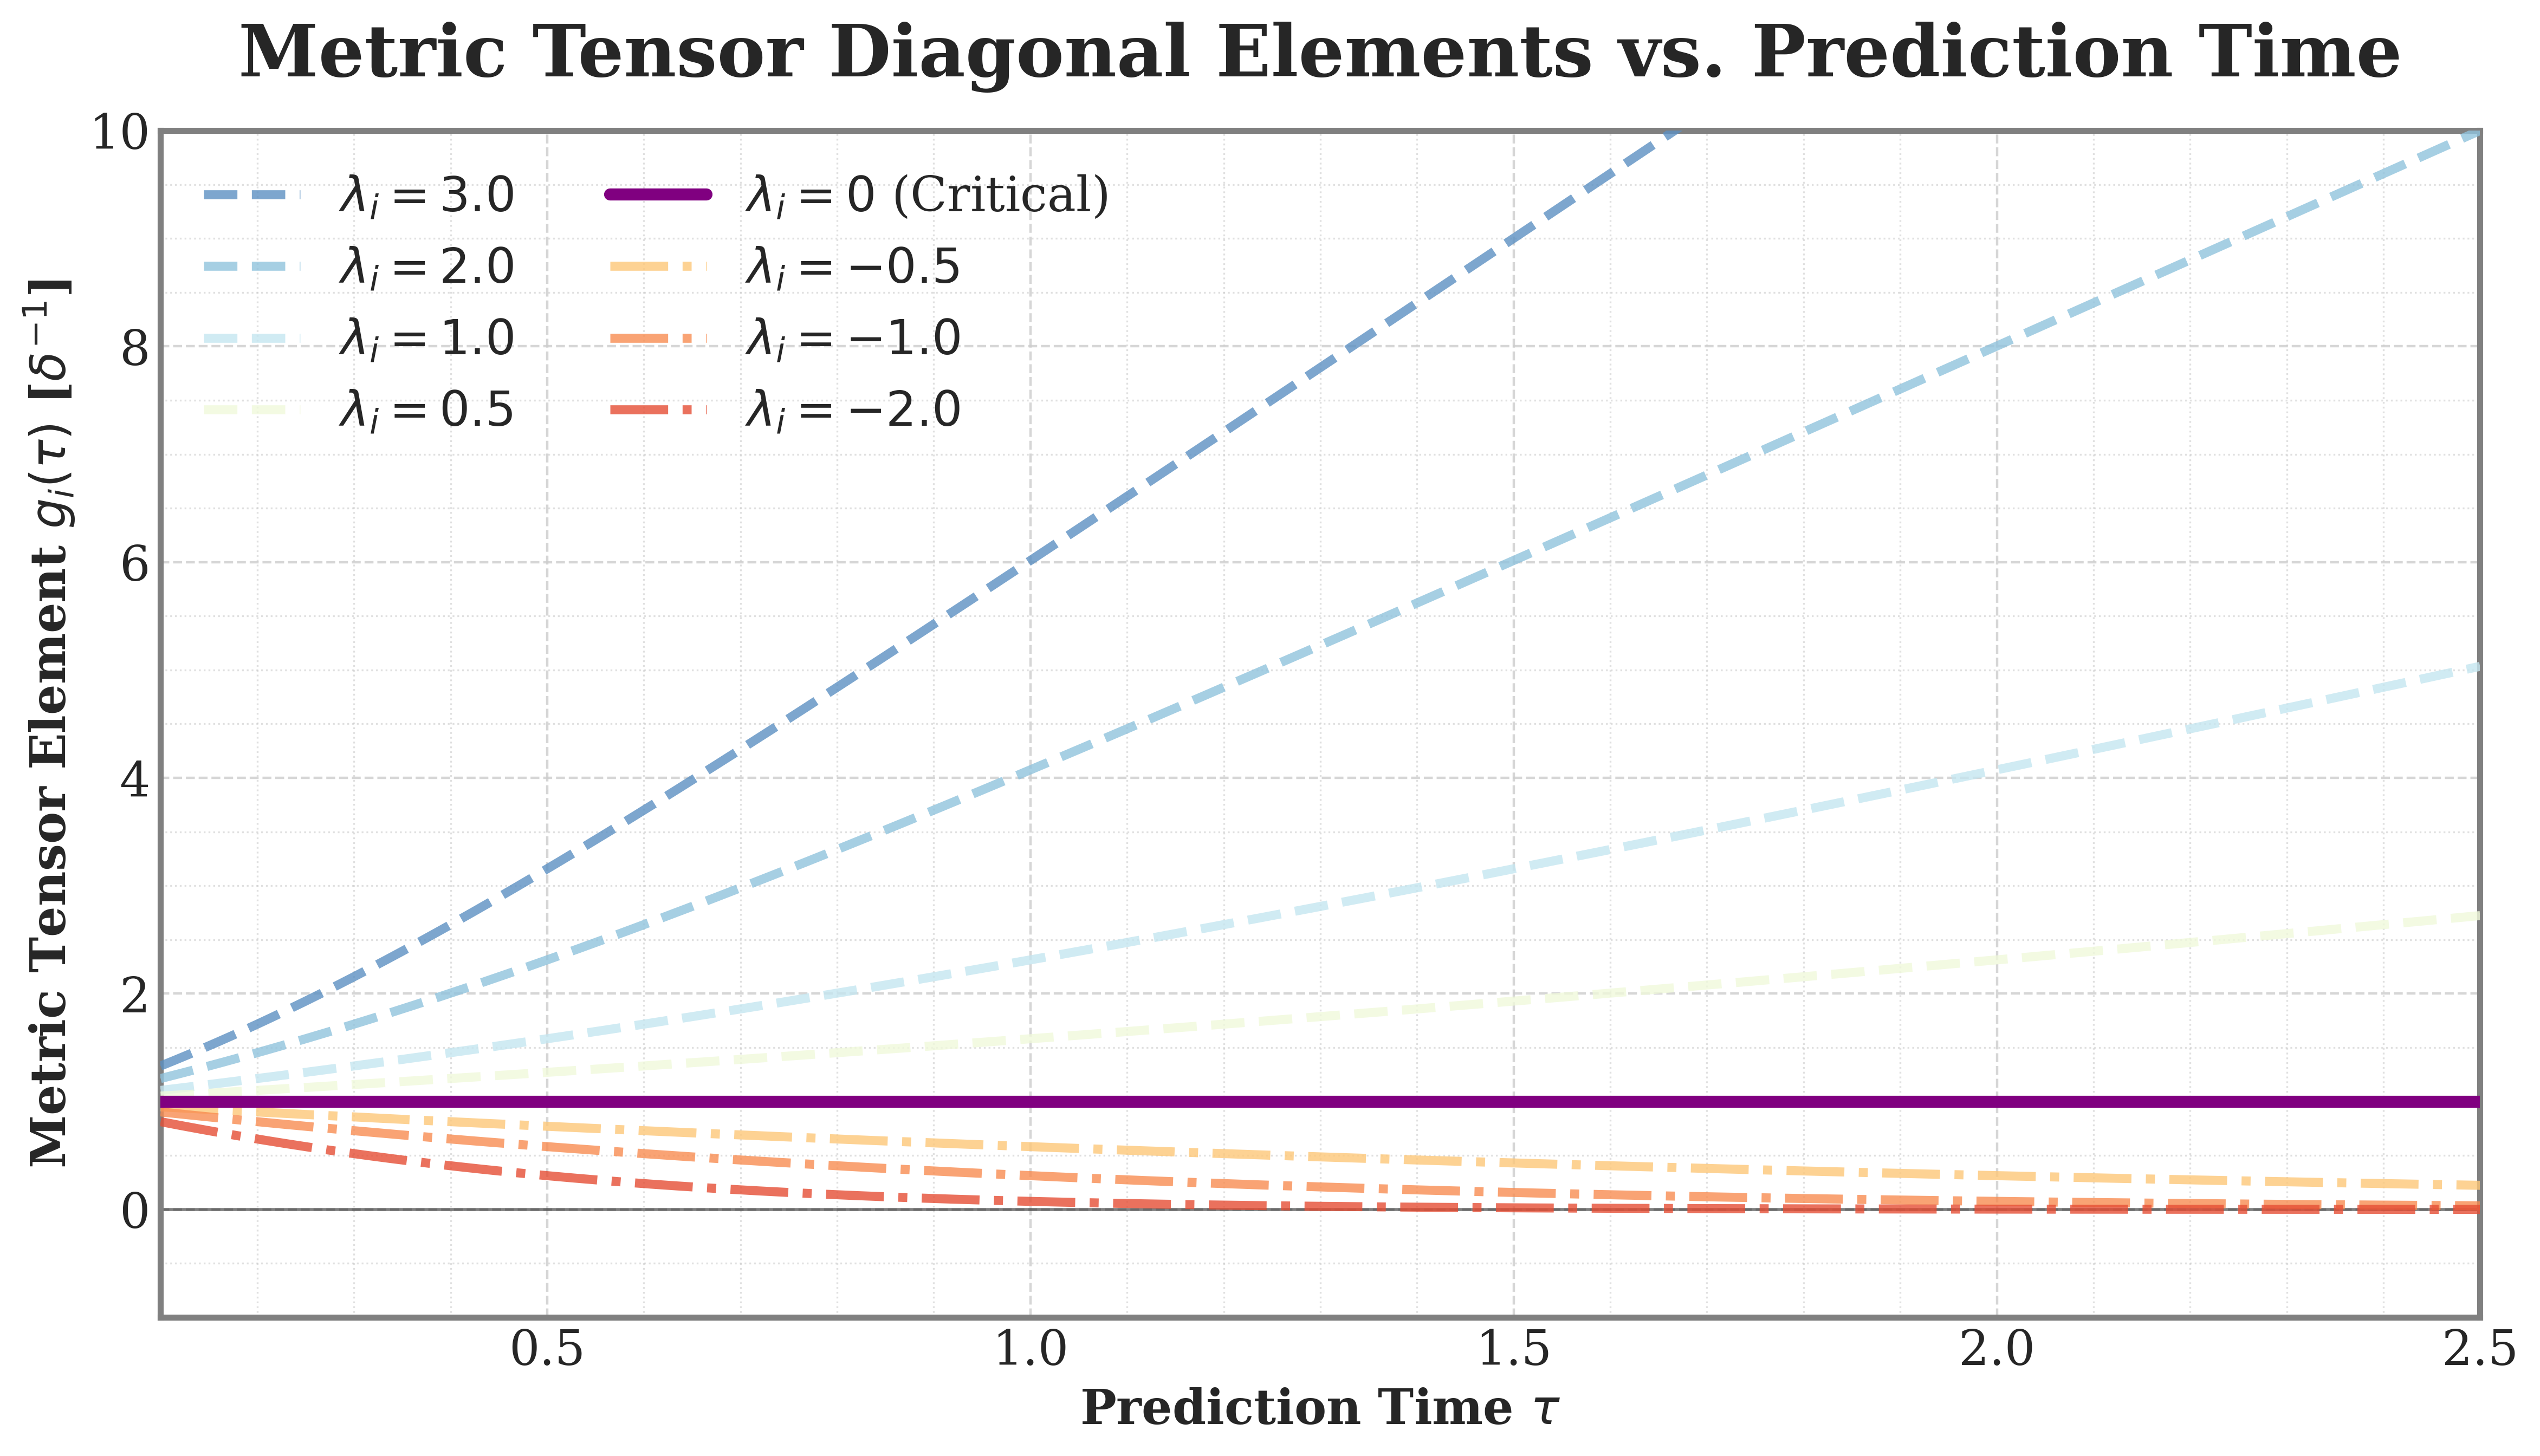
\includegraphics[width=1.00\textwidth]{./assets/Metric_Tensor_Diagonal_Elements_vs._Prediction_Time.png}
    \caption{度量张量对角元素随预报时间的演化规律}
    \label{fig:metric_vs_tau}
\end{figure}

\textbf{1. 中性方向: $\eigenval_i = 0$ (流形切方向)}

当 $\eigenval_i = 0$ 时，对应于动力学系统的\textbf{中性方向}，在该方向上初始扰动既不增长也不衰减。
此类情况通常代表系统的守恒量或近似守恒量，以及吸引子流形的切空间方向。
可预报性可以在该方向上保持较长时间。

度量对角元在 $\eigenval_i = 0$ 处需要特别处理。
利用L'Hôpital法则:
\begin{equation}
\label{eq:metric_tensor_diagonal_element_neutral}
    [\metric_{\predtime}]_{ii} = \lim_{\eigenval_i \to 0} \frac{2 \eigenval_i \predtime}{\delta_i} \cdot \frac{e^{2 \eigenval_i \predtime}}{e^{2 \eigenval_i \predtime} - 1} = \frac{1}{\delta_i}
\end{equation}

如图 \ref{fig:metric_vs_tau} 所示，中性方向的度量保持为常数。
曲率在该方向上为零，可以理解为流形上的一片“平坦区域”。
在这里不存在混沌效应的作用，动力学距离完全由扩散效应控制。
时间权重因子 $\predtime$ 恰好抵消了扩散导致的 $\predtime^{-1}$ 衰减。

中性方向对应\textbf{准守恒模态}，如地转平衡态中的位涡守恒方向、绝热过程中的熵守恒方向。
在气候尺度，海洋的盐度-温度补偿关系形成近似的中性方向。

\textbf{2. 稳定方向: $\eigenval_i < 0$ (吸引子方向)}

当 $\eigenval_i < 0$ 时，对应于动力学系统的\textbf{稳定方向}，初始扰动沿此方向指数衰减。
此类方向代表相空间中的\textbf{吸引子 (Attractor)}，是系统长时间演化的最终归宿。

设 $\eigenval_i = -\meanval_i$，其中 $\meanval_i > 0$。
度量对角元为:
\begin{equation}
\label{eq:metric_tensor_diagonal_element_stable}
    [\metric_{\predtime}]_{ii} = \frac{2 \meanval_i \predtime}{\delta_i} \frac{e^{-2 \meanval_i \predtime}}{1 - e^{-2 \meanval_i \predtime}}
\end{equation}

如图 \ref{fig:metric_vs_tau} 所示，稳定方向的度量呈指数下降，直至趋于零。
曲率在该方向上为正，可以理解为流形上的一片“碗状区域”。
沿稳定方向的初值扰动迅速衰减，两条初始接近的轨迹将以指数速率收敛至同一吸引子。
这意味着该方向上的不确定性对未来状态的影响会逐渐消失，被吸引子的收缩性所抵消。

稳定方向对应大气中的摩擦耗散、辐射冷却、海洋中的深层混合等过程。
例如，边界层湍流摩擦导致近地风速扰动快速衰减 ($\meanval \sim 1\,\text{day}^{-1}$)。
吸引子的存在保证了气候系统的\textbf{韧性 (Resilience)}: 即使遭受一定程度的外部冲击，地球系统最终仍将恢复到吸引子上。

\textbf{3. 不稳定方向: $\eigenval_i > 0$ (排斥子方向)}

当 $\eigenval_i > 0$ 时，对应于动力学系统的\textbf{不稳定方向}，通常代表相空间中的\textbf{排斥子 (Repellor)} 或鞍点上的不稳定子流形。
雅可比矩阵 $\jacobian_{\drift}$ 的正特征值表征初始扰动的指数增长率 (即Lyapunov指数)，是\textbf{混沌效应 (Chaos Effect)}的动力学根源。

度量对角元为:
\begin{equation}
    \label{eq:metric_tensor_diagonal_element_unstable}
    [\metric_{\predtime}]_{ii} = \frac{2 \eigenval_i \predtime}{\delta_i} \frac{e^{2 \eigenval_i \predtime}}{e^{2 \eigenval_i \predtime} - 1}
\end{equation}

如图 \ref{fig:metric_vs_tau} 所示，不稳定方向的度量呈线性增长趋势。
当预报时间 $\predtime$ 较长时，有 $e^{2\eigenval_i\predtime} \gg 1$，因此 $[\metric_{\predtime}]_{ii} \approx \frac{2\eigenval_i \predtime}{\delta_i}$，度量随时间线性、正比例地增长。
比例系数 $\frac{2\eigenval_i}{\delta_i}$ 可作为内禀的可预报性因子，量化动力学混沌效应与随机噪声扩散的竞争。

曲率在该方向上为负，且绝对值将随着预报时间 $\predtime$ 的增大而线性增大，像是流形上一片正在被不断扭曲的“鞍形区域”。
这是Lorenz \cite{lorenz1963deterministic} 提出的“蝴蝶效应”的微分几何表述。
系统的可预报性将随着预报时间的拉长而迅速降低，成为预报技巧损失的主导因素。

不稳定方向对应大气动力学中的\textbf{正压不稳定}和\textbf{斜压不稳定}模态。
初始扰动沿此方向呈指数增长，表现为天气尺度扰动的快速发展 (如锋生、气旋加深) \cite{palmer1993extended}。



\section{作为概率流形的气候}

\subsection{对气候变化的数学建模}

地球系统由快变量 $\fastvar$ 和慢变量 $\slowvar$ 共同描述。
快变量演化遵循Itô SDE \eqref{eq:sde}，而慢变量在天气时间尺度上近似不变。
我们认为，\textbf{气候的本质是以慢变量为参数的概率流形族}。

\begin{definition}[气候]
\label{def:climate}
    在固定慢变量 $\slowvar$ 下，气候是概率流形三元组:
    \begin{equation}
    \label{eq:climate_triple}
        \mathrm{Clim}(\slowvar) = (\manifold_{\slowvar}, \metric_{\slowvar}, \measure_{\slowvar})
    \end{equation}

    其中，$\manifold_{\slowvar}$ 是由约束定义的低维状态流形，$\metric_{\slowvar}$ 是黎曼度量，而 $\measure_{\slowvar}$ 是由随机动力学导出的不变概率测度。
\end{definition}

\begin{definition}[天气]
\label{def:weather}
    天气是快变量在气候流形 $\mathrm{Clim}(\slowvar)$ 上的一次随机轨迹 $\{\fastvar_t\}_{t \in [0, T]}$，即按照Itô SDE \eqref{eq:sde} 采样得到的一条路径。
\end{definition}

\textbf{气候变化 (Climate Change)}是由慢变量 $\slowvar(t)$ (如温室气体浓度、太阳辐射、冰盖体积) 演化驱动的概率流形三元组的时间依赖过程:
\begin{equation}
\label{eq:climate_change_evolution}
    \mathrm{Clim}(\slowvar(t)) = (\manifold_{\slowvar(t)}, \metric_{\slowvar(t)}, \measure_{\slowvar(t)}), \quad t \in [t_0, t_1]
\end{equation}

\begin{definition}[吸引子]
\label{def:attractor}
    设动力系统 $\frac{d\fastvar}{dt} = \drift(\fastvar; \slowvar)$ 在流形 $\manifold_{\slowvar}$ 上演化。
    集合 $\attractor_{\slowvar} \subset \manifold_{\slowvar}$ 称为吸引子，若其是概率测度$\measure_{\slowvar}$ 的支撑集: $\attractor_{\slowvar} = \mathrm{supp}(\measure_{\slowvar})$。
    即 $\measure_{\slowvar}(\attractor_{\slowvar}) = 1$ 且 $\attractor_{\slowvar}$ 是满足此条件的最小闭集。
\end{definition}

根据吸引子的拓扑结构是否改变，我们可以将气候变化分为两类。

\subsection{I类气候变化: 概率测度的演化}

\begin{definition}[I类气候变化]
\label{def:type1_climate}
    若慢变量 $\slowvar(t)$ 在时间区间 $[t_0, t_1]$ 内演化，气候吸引子 $\attractor_{\slowvar(t)}$ 满足拓扑不变性:
    \begin{equation}
        H_*(\attractor_{\slowvar(t)}) \cong H_*(\attractor_{\slowvar(0)}), \quad \pi_0(\attractor_{\slowvar(t)}) = \text{const}, \quad \forall t \in [t_0, t_1]
    \end{equation}

    而流形度量 $\metric_{\slowvar(t)}$ 和概率测度 $\measure_{\slowvar(t)}$ 连续演化，则称系统发生I类气候变化。
\end{definition}

I类气候变化是当前气候系统的主要演化模式。
我们首先说明，在I类变化中，吸引子拓扑保持不变，流形与度量的演化缓慢且效应不显著，但概率测度 $\measure_{\slowvar}$ 可以发生较显著的改变。

稳态Fokker-Planck方程 \eqref{eq:steady_fp} 的解 $\probdens_{ss}$ 由向量场 $\drift$ 和扩散张量 $\difftensor$ 决定。
考虑一维系统，不变概率测度满足:
\begin{equation}
\label{eq:steady_fp_solution}
    \probdens_{ss}(x; \slowvar) \propto \frac{1}{\difftensor(x; \slowvar)} \exp\left(\int^x \frac{\drift(y; \slowvar)}{\difftensor(y; \slowvar)} dy\right)
\end{equation}

对 $\drift$ 求偏导:
\begin{equation}
\label{eq:sensitivity_mean_partial_f}
    \frac{\partial \probdens_{ss}}{\partial \drift} = \probdens_{ss}(x) \cdot \frac{\partial}{\partial \drift}\left[\int^x \frac{\drift(y)}{\difftensor(y)} dy\right] = \probdens_{ss}(x) \cdot \int^x \frac{1}{\difftensor(y)} dy
\end{equation}

对 $\difftensor$ 求偏导:
\begin{equation}
\label{eq:sensitivity_mean_partial_d}
    \frac{\partial \probdens_{ss}}{\partial \difftensor} = \probdens_{ss} \left[-\frac{1}{\difftensor} - \int^x \frac{\drift(y)}{\difftensor^2(y)} dy\right]
\end{equation}

均值 $\meanval$ 和方差 $\variance$ 对 $\drift, \difftensor$ 的敏感性分别为:
\begin{align}
\label{eq:sensitivity_mean}
    \frac{\partial \meanval}{\partial \drift} &= \int x \cdot \frac{\partial \probdens_{ss}}{\partial \drift} dx \sim O(1/\difftensor), \quad \frac{\partial \meanval}{\partial \difftensor} = \int x \cdot \frac{\partial \probdens_{ss}}{\partial \difftensor} dx \sim O(1/\difftensor^2) \\
\label{eq:sensitivity_variance}
    \frac{\partial \variance}{\partial \drift} &= \int (x - \meanval)^2 \frac{\partial \probdens_{ss}}{\partial \drift} dx \sim O(1/\difftensor), \quad \frac{\partial \variance}{\partial \difftensor} = \int (x - \meanval)^2 \frac{\partial \probdens_{ss}}{\partial \difftensor} dx \sim O(1/\difftensor^2)
\end{align}

向量场 $\drift$ 的微小改变 ($\Delta \drift$) 会导致均值和方差以 $O(1/\difftensor)$ 的速率变化；扩散系数 $\difftensor$ 的微小改变 ($\Delta \difftensor$) 会导致均值和方差以 $O(1/\difftensor^2)$ 的速率变化。
由于噪声强度 $\difftensor$ 相对较小，这意味着均值和方差对动力学参数的变化高度敏感。
动力学的微扰通过Fokker-Planck方程被“放大”为统计量的显著变化，
这是对气候变化非线性效应的动力学解释。

气候流形概率测度 $\measure_{\slowvar}$ 的改变将对人类社会产生直接和重要的影响，尤其是尾部概率的变化，体现为\textbf{极端事件}频率的指数增长。

设 $\climind: \manifold \to \R$ 为气候指标 (温度、降水强度、风速等)，定义极端事件为 $\climind(\fastvar) > \threshold$ ($\threshold$ 为高阈值)。
其发生概率由不变测度 $\probdens_{ss}$ 决定:
\begin{equation}
\label{eq:extreme_prob}
    P_{\text{extreme}}(\threshold; \slowvar) = \measure_{\slowvar}(\{\fastvar \in \manifold_{\slowvar} : \climind(\fastvar) > \threshold\}) = \int_{\climind(\fastvar) > \threshold} \probdens_{ss}(\fastvar; \slowvar) \, d\fastvar
\end{equation}

对应的\textbf{重现期}为:
\begin{equation}
\label{eq:return_period}
    T_{\text{return}}(\threshold; \slowvar) = \frac{1}{P_{\text{extreme}}(\threshold; \slowvar)}
\end{equation}

慢变量变化 $\slowvar \to \slowvar'$ 导致概率测度的变化。
假设 $\probdens_{ss}(\fastvar; \slowvar)$ 近似为正态分布，均值 $\meanval(\slowvar)$、方差 $\variance(\slowvar)$，则极端事件概率满足:
\begin{equation}
\label{eq:extreme_prob_normal}
    P_{\text{extreme}}(\threshold; \slowvar) \approx \frac{1}{2}\mathrm{erfc}\left(\frac{\threshold - \meanval(\slowvar)}{\sqrt{2}\sqrt{\variance(\slowvar)}}\right) \sim \exp\left(-\frac{(\threshold - \meanval(\slowvar))^2}{2\variance(\slowvar)}\right), \quad \threshold \gg \meanval
\end{equation}

若均值变化 $\meanval(\slowvar') = \meanval(\slowvar) + \Delta \meanval$ 时 ($\Delta \meanval > 0$, 方差不变)，尾部概率的相对变化为:
\begin{equation}
\label{eq:extreme_prob_mean_shift}
    \frac{P_{\text{extreme}}(\threshold; \slowvar')}{P_{\text{extreme}}(\threshold; \slowvar)} \approx \exp\left(\frac{(\threshold - \meanval)\Delta \meanval}{\variance}\right)
\end{equation}

由于 $\threshold \gg \meanval$，$\Delta \meanval$ 将导致极端事件发生的概率指数增长。

若方差变化 $\variance(\slowvar') = \variance(\slowvar) + \Delta \variance$ 时 ($\Delta \variance > 0$, 均值不变)，尾部概率变化为:
\begin{equation}
\label{eq:extreme_prob_variance_increase}
    \frac{P_{\text{extreme}}(\threshold; \slowvar')}{P_{\text{extreme}}(\threshold; \slowvar)} \approx \exp\left(\frac{(\threshold - \meanval)^2 \Delta \variance}{2(\variance)^2}\right)
\end{equation}

方差增大使概率测度尾部加厚，即分布更加扁平，极端值的概率密度将会更高。
由于 $\threshold \gg \meanval$，$\Delta \variance$ 亦将导致极端事件发生的概率指数增长。

近年来，人类活动导致的气候变化已经导致了极端事件频率的显著增加。
以\textbf{全球变暖}为例，$\text{CO}_2$ 浓度升至 $420$ ppm，全球温度均值升高 $1.1$ °C、方差增加 $15\%$。
IPCC AR6报告显示 \cite{ipcc2021ar6}，$1.5$ °C的增温将使千年一遇的极端热浪变为百年一遇，$P_{\text{extreme}}$ 增加 $10$ 倍，这正是均值和方差变化带来的指数增长效应。

\subsection{II类气候变化: 拓扑突变与临界转变}

\begin{definition}[II类气候变化]
\label{def:type2_climate}
    若慢变量跨越临界值 $\slowvar^*$ 时，气候吸引子的拓扑结构发生间断改变:
    \begin{equation}
        H_*(\attractor_{\slowvar_-}) \not\cong H_*(\attractor_{\slowvar_+}), \quad \text{或} \quad \pi_0(\attractor_{\slowvar_-}) \neq \pi_0(\attractor_{\slowvar_+}), \quad \text{或} \quad \dim_H(\attractor_{\slowvar}) \text{跳跃}
    \end{equation}

    其中 $\slowvar_{\pm} = \slowvar^* \pm \epsilon$，则称系统发生II类气候变化，$\slowvar^*$ 为临界点 (Tipping Point)。
\end{definition}

II类变化对应动力系统的\textbf{分岔}。
在临界点 $\slowvar^*$ 处，向量场 $\drift_{\slowvar}$ 的雅可比矩阵至少有一个特征值穿越虚轴 ($\mathrm{Re}(\eigenval) = 0$)。
这将导致度量张量发生退化，意味着吸引子的稳定性转移或拓扑结构改变，如吸引子消失 (Saddle-node分岔)、周期轨道产生 (Hopf分岔)、对称破缺 (Pitchfork分岔) 等。

接近临界点时，系统将在多个层面呈现出可测量的\textbf{预警信号 (Early Warning Signals)} \cite{scheffer2009early}:
\begin{itemize}
    \item \textbf{临界慢化 (Critical Slowing Down)}:
    系统对扰动的恢复时间 $\predtime \sim 1/\sqrt{\eigenval} \to \infty$。
    具体表现为主导衰减模式的松弛率 $\eigenval_{\text{relax}} = -\mathrm{Re}(\eigenval_{\text{leading}}) \to 0^+$。
    \item \textbf{自相关增强 (Autocorrelation Enhancement)}:
    时间序列的滞后-1自相关系数趋近于1: $\mathrm{AC}(1) = \mathrm{Corr}(x_t, x_{t-1}) \to 1$，表明系统的“记忆”增强，状态转移减慢。
    临界点处 $\mathrm{AC}(1) \approx 1 - 2\eigenval_{\text{relax}}\Delta t$，可用于估计距临界点的距离。
    \item \textbf{方差发散}:
    概率测度向鞍点附近集中，导致状态变量的方差趋于无穷: $\mathrm{Var}[\fastvar] \to \infty$。
\end{itemize}

2009年，Rockström等学者提出了行星边界理论 (Planetary Boundaries theorem) \cite{rockstrom2009planetary}，认为地球系统存在9个临界子系统，即存在9个气候流形上的吸引子正在接近临界点 $\slowvar^*$。
这一理论为理解地球系统的稳态特性与气候变化的临界点提供了重要框架。

对于II类气候变化，我们介绍\textbf{大西洋经向翻转环流 (Atlantic Meridional Overturning Circulation, AMOC)} 的潜在崩溃作为典型案例。
AMOC是全球气候系统的关键组分，通过将热带暖水输送至北大西洋并驱动深层冷水南下，调节全球热量分布。
其驱动力来自北大西洋的密度差——表层海水在高纬度冷却增密并下沉，形成深层返流。然而，格陵兰冰盖融化释放的淡水正在降低海水盐度，从而减弱密度梯度并削弱环流强度。
当淡水通量超过临界阈值 $F^* \sim 0.1$ Sv时，系统将跨越临界点。

从拓扑结构来看，AMOC存在两个吸引子态: “强翻转”态 ($\sim 20$ Sv，当前态) 和“弱翻转/关闭”态 ($< 5$ Sv)。
这对应两个独立的吸引子盆地 ($\pi_0 = 2$)。
临界点处，“强翻转”盆地在相空间中收缩至零测度集，随后消失 ($\pi_0: 2 \to 1$)，系统被迫不可逆跃迁至“关闭”态。
数学上，这是一个\textbf{Saddle-node分岔}，吸引子与鞍点在临界流形上碰撞湮灭。

观测数据为这一理论预测提供了有力支持。
Ditlevsen \& Ditlevsen (2023) \cite{ditlevsen2023warning} 分析了1870-2020年间的AMOC指标 (海温梯度、盐度剖面)，发现了多个临界预警信号。
自相关系数从1950年代的 $\mathrm{ACF}(1) \approx 0.7$ 增至2020年的 $\approx 0.9$，增幅达 $0.2$，这对应着松弛时间从 $20$ 年延长至 $100$ 年。
同时，方差增长率 $d\mathrm{Var}/dt > 0$ 且在1970年代后加速，符合临界慢化理论的预测。
基于这些信号，统计模型估计AMOC可能在2040-2070年间跨越临界点 ($95\%$置信区间)。

AMOC崩溃的全球影响将是灾难性的。
北欧地区将因失去暖流输送而温度下降 $3-5$ °C；热带辐合带将因大气环流重组而南移；美国东海岸将因海洋动力学高度变化而经历 $30-50$ cm的海平面上升；亚马逊和非洲萨赫勒地区将因远程气候耦合而降水减少 $20-40\%$。
这些变化对应着地球系统吸引子流形的拓扑重构，将影响数十亿人的生存环境。

\subsection{遥相关}

地球气候系统展现出显著的\textbf{空间遥相关 (Remote Correlation)}现象: 空间上相隔数千公里的区域，其气候变率却呈现出强相关性。
以ENSO为例 \cite{trenberth1997definition}，赤道东太平洋的海表温度异常不仅影响南美洲西海岸，还与北美冬季降水、东亚夏季风、澳大利亚干旱等全球气候模式存在显著关联，相关系数可达 $r > 0.5$。
类似地，NAO指数与欧洲冬季温度和降水模式密切相关 \cite{hurrell1995decadal}，而PDO影响着整个太平洋盆地的气候变率 \cite{mantua1997pacific}。
这些跨越地理尺度的联系挑战了传统的局域因果观念，需要从气候流形的角度理解。

\begin{definition}[遥相关]
\label{def:remote_correlation}
    设气候流形 $\manifold$ 上的状态空间 $\mathbb{R}^N$ 存在空间位置索引 $i \in \{1, 2, \ldots, N\}$，每个位置对应一个坐标映射 $x_i: \manifold \to \mathbb{R}$。
    称位置 $i$ 与 $j$ 存在遥相关，若满足:
    \begin{equation}
        |\mathrm{Corr}_{\measure}[x_i, x_j]| > \epsilon, \quad \text{且} \quad \|\bm{r}_i - \bm{r}_j\| \gg L_c
    \end{equation}

    其中 $\bm{r}_i, \bm{r}_j$ 为空间位置坐标，$L_c$ 为系统特征空间尺度，$\epsilon$ 为显著性阈值，$\measure$ 为气候流形上的概率测度。
\end{definition}

遥相关可以通过流形上的模态分解精确刻画。
设气候流形嵌入为 $\iota: \manifold \to \mathbb{R}^N$，任意气候状态可分解为:
\begin{equation}
\label{eq:modal_decomposition}
    \fastvar(t) = \bar{\fastvar} + \sum_{k=1}^K a_k(t) \mode_k, \quad K \ll N
\end{equation}

其中 $\{\mode_k\}$ 是流形的主方向 (对应经验正交函数EOF或主成分PC模态)，$a_k(t)$ 是时间演化的模态系数，$K$ 是有效维度。
两个空间位置的协方差可以表示为:
\begin{equation}
\label{eq:covariance_between_two_points}
    \mathrm{Cov}_{\measure}[x_i, x_j] = \sum_{k=1}^K \eigenval_k \phi_k^{(i)} \phi_k^{(j)}
\end{equation}

其中 $\eigenval_k$ 是第 $k$ 个模态的方差贡献，$\phi_k^{(i)}$ 是模态 $\mode_k$ 在位置 $i$ 的空间投影。

\eqref{eq:covariance_between_two_points} 揭示了遥相关的代数结构: 即使位置 $i$ 和 $j$ 在地理上相隔遥远（$\|\bm{r}_i - \bm{r}_j\| \gg L_c$），只要它们在同一主模态 $\mode_k$ 上的投影 $\phi_k^{(i)}$ 和 $\phi_k^{(j)}$ 同时显著，就会产生强相关。
这一现象的根本原因在于气候流形的内在低维性 (流形假设 \ref{ass:manifold_hypothesis})。

地球系统中的遥相关也可以用气候流形的曲率来进一步阐释。
正曲率对应于吸引子方向 (测地线收缩)，负曲率对应于排斥子方向 (测地线发散)。
当流形存在低维吸引子 ($K \ll N$) 时，在大部分方向上具有正曲率并快速收缩，只有少数不稳定方向上具有负曲率。
遥相关正是这种几何收缩的统计表现: 尽管初始状态空间是高维的 ($\dim = N$)，但由于大部分方向因吸引子作用而快速收缩，概率测度 $\measure$ 集中在由少数主模态张成的低维子流形上。
因此，当我们观测不同位置的坐标映射 $x_i$ 和 $x_j$ 时，它们的变化实际上都反映了流形在这些低维方向上的演化，从而产生显著的远程统计相关性。



\newpage
\bibliographystyle{unsrtnat}
\bibliography{references}

\end{document}
